%!TEX root = ../template.tex
%%%%%%%%%%%%%%%%%%%%%%%%%%%%%%%%%%%%%%%%%%%%%%%%%%%%%%%%%%%%%%%%%%%
%% chapter1.tex
%% NOVA thesis document file
%%
%% Chapter with introduction
%%%%%%%%%%%%%%%%%%%%%%%%%%%%%%%%%%%%%%%%%%%%%%%%%%%%%%%%%%%%%%%%%%%

%Before chapter reordering:
%Taking into account the existing usability problems and the target users' requirements and expectations, a methodology was essential in order to design, implement, and evaluate solutions throughout the development process. Therefore, this chapter will present the multiple phases and techniques carried out since the first sketches to the final evaluations.

\chapter{Methodologies}
\label{cha:methodologies}
The problem approached in this dissertation required a reformulation of the visual interface used to query data. As such, the methodology used to design, implement and evaluate each phase of the solution development was regarded as a key factor to keep the right focus until reach the final stage. 

In that way, this chapter will present an overview of the methodology adopted as well as how users were integrated into the process in order to maintain a user-centered design approach.

\section{Problem Exploration}
\label{sec:problem_exploration}

Even though there was a general idea of the problems of the existing interface, a complete plan was designed to perform a deep exploration of the aforementioned problems. The main concern was to obtain a global and complete view of the problems through different gathering strategies in order to examine the problem from different perspectives rather than using only a subset of users or data, which could bias the problems' perception.

%The first stage contemplated was a deep exploration of the problems of the existing interface. Although there was a general idea of the existing usability problems of the interface, a plan following different gathering strategies was thought to examine the problem from different perspectives rather than using only a subset of users or data, which could bias the problems' perception.

Firstly, the existing problems were identified in a wide sense from the perspective of a user who does not have context about how the query builder works, in order to realize the difficulties that new users who tried to start using the interface could feel. After that, other gathering techniques were applied in order to perceive also the problems felt by expert users and progressively understand the most detailed aspects of the problems presented. Therefore, the methods presented below, which will be further detailed in section \ref{sec:problem_analysis}, were applied, in this order, to obtain a wide and diverse view of the existing problems: 

\begin{itemize}
    \item \textbf{Analysis: } Visualization of the OutSystems tutorials regarding data querying and self-exploration of the interface in order to analyze and identify a preliminary set of preliminary problems;
    \item \textbf{User Interviews: } Simple and direct dialogues with end-users of the OutSystems platform to listen their opinion concerning the query builder. The main aim was to notice in which reasons they use it, what are their major difficulties using it, or even the struggles or barriers which make them to not use it; 
    \item \textbf{Data Analysis: } Analysis of the queries formulated in \gls{SQL} through the OutSystems Platform extensibility feature which allow developers to add queries in \gls{SQL} to perceive if \gls{SQL} is used only for advanced used cases not supported by the visual query, or if it is often used to cover simple use cases;
    \item \textbf{Community Ideas: } Exploration of the discussions in the forums of the OutSystems Community regarding data querying to aggregate more information about problems users feel and suggestions to improve it;
    \item \textbf{Existing Interface Evaluation: } Usability tests to the existing interface in order to visualize directly how users interact with the system as well as what they feel when trying to understand and formulate database queries using the visual query builder. The results of this problem information gathering would promote also important results to validate the further prototypes since it would be possible to compare the usability of the new prototypes with the existing interface.
\end{itemize}

\section{User Analysis}
\label{sec:user_analysis}
As mentioned, an user-centered design approach was applied and hence an analysis of the target users of the system, which will be further presented in section\ref{sec:target_users}, was performed to perceive and categorize the users who use the query builder. In this analysis, the users were classified and divided into three groups: OutSystems Developer, Software Developer, and Citizen Developer.

In that way, the topics that could most branch out the users' requirements and expectations were pointed out to perceive how users could be divided into different groups. These groups were used throughout the design process to characterize the target users of the system. Each group represents a subset of the system's users, which should be separated from the remaining ones due to their user's profiles. Henceforth, all usability tests were performed in an equitable manner with users of all groups in order to obtain a representative sample of the end-users of the system.


\section{Iterative Design}
\label{sec:iterative_design}
After comprehending the existing problems and the target users of the system, the phases for the sake of the design and development of the final solution were planned. Accordingly, the design strategy adopted, which will be further detailed in Chapter \ref{cha:design_and_implementation}, will be briefly presented. The chosen methodology used an iterative design strategy in order to keep a user-centric design, which prioritizes the users' needs according to the mentioned in section \ref{subsec:user_centered_design}.

%Nevertheless, there was the demand to deeply analyze the problem reach a more complete defined list of the requirements.

\textbf{Sketching: }The design process started with an initial sketching phase, where the first solution ideas were explored and drafted. In this technique, the integration of new ideas into the existing interface is favored given the fact it is an interactive process where the ideas are tested progressively. The most important aspect was to think about system transversal changes and not about particular details of specific components, since these details could be refined later. The outcome of this phase sets a more concrete idea of what can be inserted in the prototype, even if it is necessary to think more about how to implement it later.

Keeping in mind the ideas explored in the sketching phase, it is possible to start to build the prototypes that will be tested by users. The evolutionary prototyping principle (described in section \ref{subsubsec:sketching_and_prototyping}) was applied. Accordingly, the last prototype was used as a baseline to develop the prototype of the next iteration. As mentioned in section \ref{subsubsec:sketching_and_prototyping}, the first prototypes should be low-fidelity prototypes, and iteration by iteration, this level should increase in order to refine details in the interface. In that way, it was decided to build two prototypes:

\begin{itemize}
    \item \textbf{Paper Prototype: } Simple low-fidelity prototype implemented in paper using a ruler, a set square, and writing materials. Through that approach, it is possible to implement the first ideas faster and reduce the risk of adoption failure, since the implemented ideas were already tested. The main concern of this type of prototype is that the design of the major interface changes might affect users mental model which enables the early detection of which choices should continue to the next iterations or if they need to be redesigned.
    \item \textbf{Service Studio Prototype: } This is the final prototype, developed using C\#, Typescript \cite{typescript}, and React \cite{react}, which is integrated in the new Design of the Service Studio. Through this prototype, the solutions implemented were validated and compared with the previous existing implementation in order to validate if the usability of the system has improved with the implemented changes.
\end{itemize}

In each one of the two above-mentioned prototypes, it was included the following phases: design, implementation, and evaluation. In the Design phase solution ideas that could be applied were set up as well as the priorities to be tackled in the prototype. The Implementation phase refers to the concrete prototype development process. Finally, in the Evaluation phase, the prototypes were tested by end-users, according to the testing approach further explained in section \ref{sec:testing_scenarios} and section \ref{sec:evaluation_method}.

Regarding evaluation, it was necessary to establish how many users should be tested in each evaluating phase. In these phases, not only the two mentioned prototypes were considered, but also the evaluation of the existing interface mentioned in section \ref{sec:existing_interface_evaluation}. 

The data extracted from the evaluation of the existing interface provides an opportunity to compare the existing usability against the usability of the final solution. Thereby, the number of users tested in the first prototype is also an important factor.

Nielsen performed several studies quantifying how many users should be tested in a usability study, leading to the conclusion that 5 users were a sufficient number for qualitative studies since it is possible to get the maximum benefit-cost ratio - "Testing with 5 people lets you find almost as many usability problems as you'd find using many more test participants" \cite{why_you_only_need_to_test_with_5_users} \cite{how_many_test_users_in_a_usability_study}. However, to perform quantitative analysis it is necessary to get at least 20 users in order to get statistical relevance \cite{how_many_test_users_in_a_usability_study}.

According to the studies mentioned, at least 5 users of each user group (described in section \ref{sec:target_users}.) should be tested since only a qualitative analysis will be performed to validate user's interaction with the applied changes. Nevertheless, some statistical results should be also subject of analysis in order to compare if the new solution provide improved usability than the existing version. Hence, it was decided to test more users in the existing implementation and in the final prototype in order to obtain enough elements to conduct a quantitative analysis. In that way, Table \ref{tab:number_of_users_tested_by_each_user_group_and_solution} shows how many users were tested by each user group and by each solution evaluated.

\begin{table}[tb]
	\caption{Number of users tested by each user group and by each solution evaluated}
	\label{tab:number_of_users_tested_by_each_user_group_and_solution}
\centering
\resizebox{\textwidth}{!}{
\begin{tabular}{c|c|c|c|c|}
    \cline{2-5}
    \rowcolor[HTML]{C0C0C0} 
    \cellcolor[HTML]{FFFFFF}                                 & Previous Implementation & Paper Prototype & Service Studio Prototype & Total \\ \hline
    \multicolumn{1}{|c|}{\cellcolor[HTML]{C0C0C0}OutSystems Developer}    & 10         & 5               & 10                    & 25 \\ \hline
    \multicolumn{1}{|c|}{\cellcolor[HTML]{C0C0C0}Software Developer} & 10        & 5              & 10                   & 25\ \\ \hline
    \multicolumn{1}{|c|}{\cellcolor[HTML]{C0C0C0}Citizen Developer} & 10        & 5              & 10                   & 25\ \\ \hline
    \multicolumn{1}{|c|}{\cellcolor[HTML]{C0C0C0}Total} & \textbf{30}        & \textbf{15}              & \textbf{30}                   & \textbf{75}\ \\ \hline
    \end{tabular}
    }
\end{table}

To compare the different phases, all tests were performed using the same testing scenarios, which are presented in the following section.


\section{Testing Scenarios}
\label{sec:testing_scenarios}
Given the wide scope of the usability problems identified, a plan of the testing approach was required in order to evaluate the most important aspects of the user-interface communication, given the short period available to test the users. Following the plan, it was possible to keep the testing focus on the prioritized details in a feasible way.

Firstly, it was defined the type of testing scenarios that would be presented. For that decision, it was taken into account the specific aspects that should be improved in the interface usability. As mentioned, not only the optimization of the efficiency, effectiveness, learnability, and user satisfaction of the entire query formulation process was the goal, but also the improvement of the query comprehension. In such a way that it was important to evaluate if users could understand the query purpose (i.e., what data intends to be fetched from the database) as well as the time they required to realize that.

Considering those evaluation requirements, two types of testing scenarios were prepared: scenarios where users explore an existing query and try to realize what was its purpose, and the other ones where users try to formulate it on their own. Through that approach, it was possible to analyze the usability of the interfaces tested for both points of view: comprehension and formulation.

Nevertheless, the complexity of the queries presents a crucial factor when the scenarios were devised. For example, an interface could be useful and pleasant to use in simple use cases but it could lead to a decrease of that quality in more complex queries. Accordingly, the requirements that were considered relevant to be covered by user testing scenarios are listed below:

\begin{itemize}
    \item \textbf{Query Comprehension: }Relevant aspects that should be present in the queries and consequently in the interface to evaluate the queries' comprehension:
    \begin{itemize}
        \item \textbf{Interface Elements Exploration: }Include use cases that contain the majority of the query components supported by the system: database entities and joins of different types, filtering and sorting criteria applied to different data types, and other query components added throughout the query formulation process, such as Group Bys, Aggregation Functions (SUM, MIN, MAX, AVG, COUNT) or Calculated Attributes \footnote{These operations were presented in section \ref{subsubsec:current_progress}};
        \item \textbf{Joins Representation: }Representation of different joins in order to analyze if users could successfully identify them. First of all, there was a concern to consider in the scenarios joins of different types, such as inner joins or left joins. It was important to consider not only the most common joins (i.e., joins where the unique foreign key referencing another table is equals to the other table primary key) but also some queries that contain joins with more advanced conditions. For instance, when the join between two tables could be made using different foreign keys, as they are multiple relationships between both tables, or when the join condition contains logical operators.
    \end{itemize}
    \item \textbf{Query Formulation and Modification: }At the same time, the following aspects were considered essential to be approached in the user testing scenarios from a query formulation or modification point of view:
    \begin{itemize}
        \item \textbf{Add Data Sources and Joins: }Identify the options chosen to add query sources and analyze what are the users' reactions to the system automatisms to simplify the joins specification;
        \item \textbf{Edit Query Filters: }Evaluate if the query filters edition is intuitive and what barriers could exist in the interfaces regarding this aspect;
        \item \textbf{Insert Calculated Attributes, Group Bys, and Aggregation Functions: }Check if users could understand the cases where they would need to use the referred functionalities and if they can discover how to apply them without difficulty;
        \item \textbf{Use Hidden Columns: }Verify the main difficulties identified by users when they need to apply actions in attributes that were not entirely visible in the interface, either because they are hidden, or because they are not visible due to the lack of available space in the interface (scroll required).
    \end{itemize}
\end{itemize}

The aspects mentioned were considered the most relevant to analyze since they allow a widespread use of the tool but they also cover multiple cases identified as critical in terms of usability, according to the aspects further detailed in section \ref{sec:problem_analysis}.

Nevertheless, the data model could have also a significant impact on user testing results. For instance, if a user does not understand the data model, he could miss the purpose of the query, even if the query is presented in a simple and readable manner. In that way, the selection of the data model used for user testing was performed attending to the following points:

\begin{itemize}
    \item \textbf{Simple Business Domain: }The data stored in the database should represent an example of a day-to-day application that could be understandable by any user regardless of his background.
    \item \textbf{Different data types: }The data model should contain a wide variety of data types since it could become useful in order to reflect if the design approaches chosen are able to work with different types of data;
    \item \textbf{Multiple relationships between two entities: }The interface aims to accelerate and simplify the querying process not only for simple cases. For this reason, it is important to perceive how the interface could help users in cases where there are more than one relationship between two entities. Moreover, \gls{SQL} does not have any particular syntax that helps users in these cases, then there is an improvement opportunity here.
\end{itemize}

\begin{figure}[htbp]
	\centering
	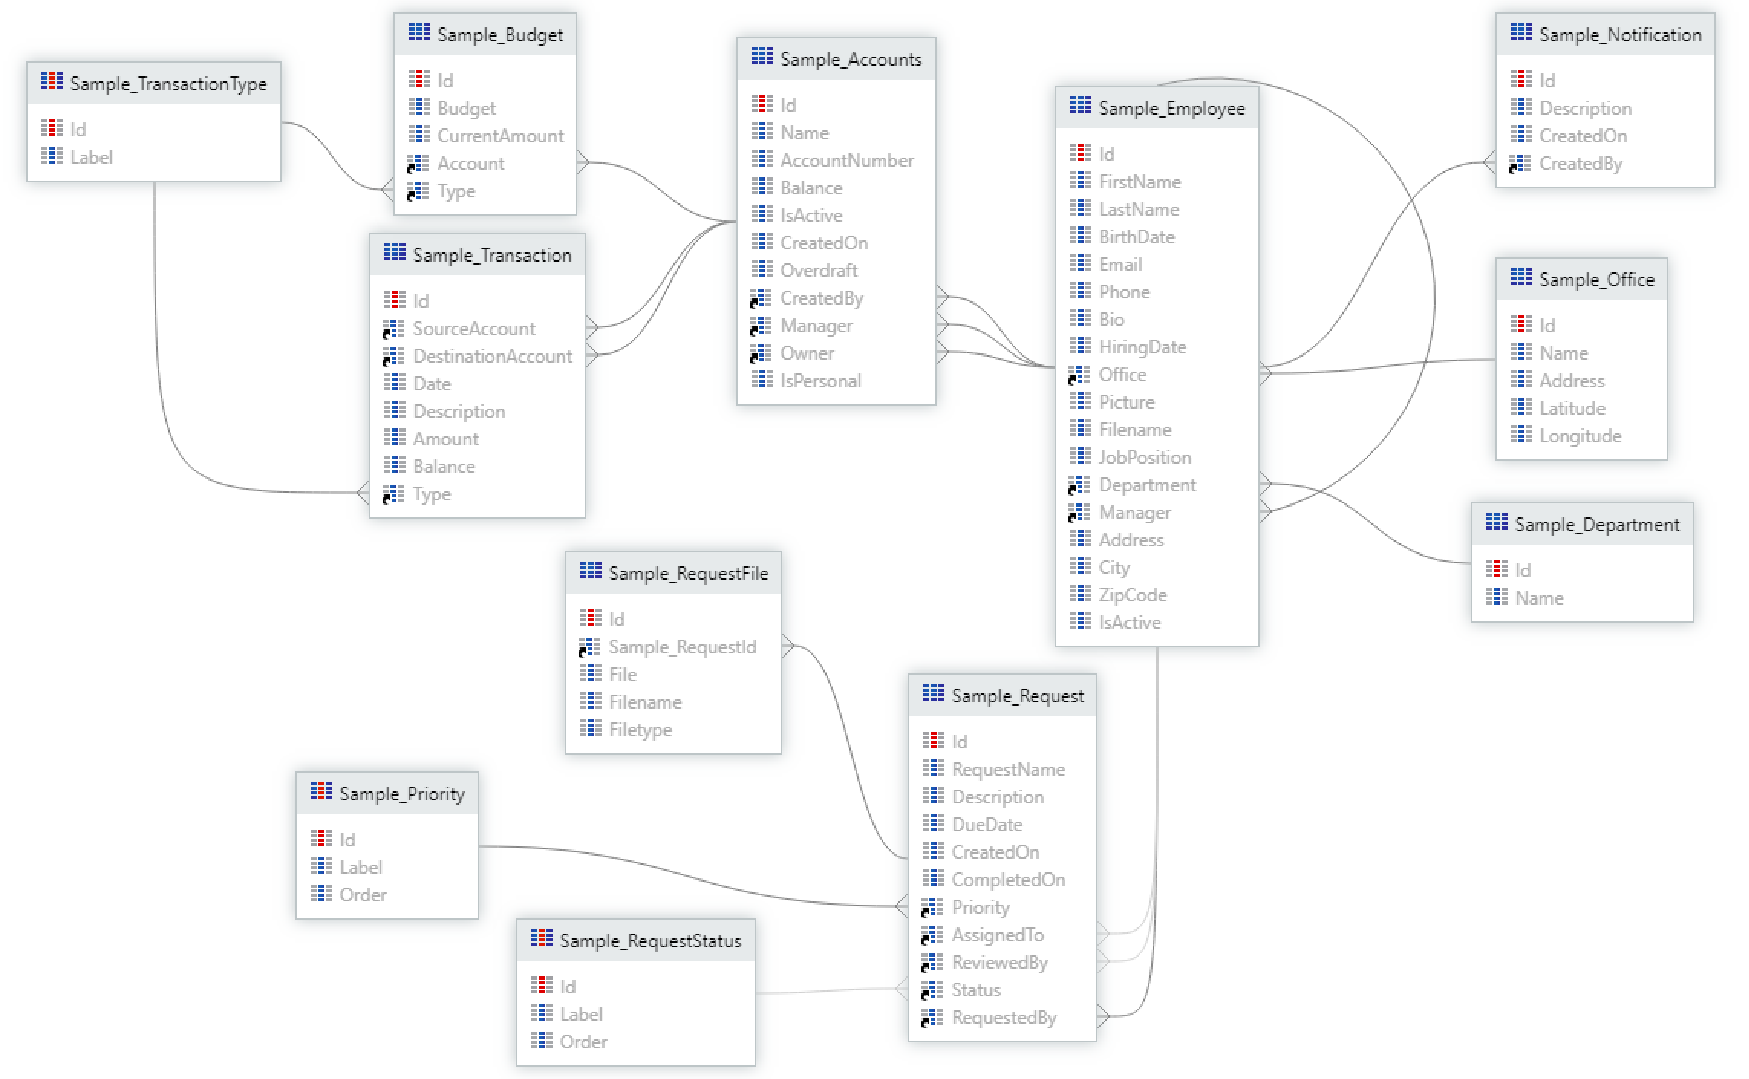
\includegraphics[height=3.6in]{data-model}
	\caption{Data Model used for User Testing}
	\label{fig:dataModel}
\end{figure}

Accordingly, \ref{fig:dataModel} illustrates the data model of the database adopted to perform all usability tests.

After choosing the data model used as support for the usability tests, the list of test scenarios was elaborated. Three different types of scenarios were designed:

\begin{itemize}
    \item \textbf{Query Comprehension: } The user explores a visual query already built and tries to indicate what are the query components presented as well as the data that would be fetched from the database through that query;
    \item \textbf{Query Modification: } After a query comprehension example, the user tries to apply some modification on the existing query previously explored;
    \item \textbf{Query Formulation: } Given a natural language statement that explains what data is intended to be fetched from the database, the user tries to formulate a new visual query from scratch in order to retrieve the data intended.
\end{itemize}

Through that approach, it was possible to keep the focus on different aspects according to the scenario used. On the one hand, the comprehension scenarios give the focus to the query readability, which promote a global exploration of the query components and gave the opportunity to understand if users clearly identified the purpose of each interface section. On the other hand, modification and formulation scenarios were used to understand if users could built queries through the interface presented.

In that way, the scenarios below, built to fetch data to the data model presented in Figure \ref{fig:dataModel}, were presented to the user in this order:  

\begin{enumerate}
    \item \textbf{Query Comprehension 1 (C1): }Employees of “Portugal” or “Japan” of departments “Services Support West” or “Services Support East” who have a job position different from “Services Representative” and never have created any notification. The employees must be presented ordered by their last name (descending order);
    \item \textbf{Query Modification 1 (M1): }Change the existing query to consider only the employees of offices "Australia" or "Japan", their department must be "Marketing" or "Services Support East", and they must have any job position. Moreover, create an attribute to present employees’ full names;
    \item \textbf{Query Comprehension 2 (C2): }List for each AccountNumber the amount sum of transactions of type “Eating Out”. Moreover, the transaction is only shown if its source account is managed by employees of department “Credit Control” and office “United Kingdom”. Account Numbers are sorted by their amount sum in descending order;
    \item \textbf{Query Comprehension 3 (C3): }List the number of employees by department and office. The number of employees is presented in descending order;
    \item \textbf{Query Formulation 1 (F1): }Notifications created by employees who are owners of a set of accounts which, at least, must combinedly average a balance of 20.000 (average of balances of accounts owned by each employee);
    \item \textbf{Query Comprehension 4 (C4): }List all requests assigned to employees of department “Services Support West” ordered by priority in the first place (“High” first), and secondly by creation date (oldest dates first);
    \item \textbf{Query Modification 4 (M4): }Considering the previous requests, change the query to show only the ones that were requested by employees from other departments (not the same).
\end{enumerate}

Nevertheless, there were several results to be obtained from the user testing scenarios and it was difficult to reach an approach to test all aspects related to the existing problems in a short period. Accordingly, Table \ref{tab:scenarios_complexity} was used to distribute the requirements mentioned across all scenarios, without turning the usability test exhaustive and heavy for users.

%Considering the short period available to test all mentioned requirements, the aspects considered essential to be present in the use cases explored were combined in a table in order to distribute them along a set of scenarios. Figure X 

%Therefore, Table \ref{tab:scenarios_complexity} was used to distribute the requirements mentioned across all scenarios presented to each user by the order presented below:



\textbf{Table \ref{tab:scenarios_complexity} clarifications regarding the factors integrated in testing scenarios: }
\begin{itemize}
    \item \textbf{Simple Joins: }Joins that are automatically generated by the system without requiring human intervention;
    \item \textbf{Complex Joins: }Joins that need to be partially configured manually (e.g., to specify the foreign key used to merge both tables or to change the join condition);
    \item \textbf{Left Join with Null: }Left join between entities A and B, to consider only the entities A that are not related to B (e.g., the employees who have not created any notification.);
    \item \textbf{Group by (without reference): } The system has an automatism that generates automatically a name to a new attribute grouped by. However, this name is not self-explanatory and there was no reference to the source of its attribute. That way, it is important to highlight this case;
    \item \textbf{Aggregation Functions: } The aggregation functions supported by aggregates are Max, Min, Average, Sum, and Count. As the representation in the interface as well as the insertion method is similar, only a few of these were used;
\end{itemize}

\begin{table}[tb]
    \caption{Distribution of the relevant testing aspects among the testing scenarios designed.}
	\label{tab:scenarios_complexity}
    \begin{tabular}{|l|l|c|c|c|c|c|c|c|}
        \hline
        \multicolumn{2}{|l|}{\textbf{Scenarios}}                                                                                                                                                          & \multicolumn{1}{l|}{\textbf{C1}}           & \multicolumn{1}{l|}{\textbf{M1}} & \multicolumn{1}{l|}{\textbf{C2}}           & \multicolumn{1}{l|}{\textbf{C3}}           & \multicolumn{1}{l|}{\textbf{F1}} & \multicolumn{1}{l|}{\textbf{C4}}           & \multicolumn{1}{l|}{\textbf{M4}} \\ \hline
                                                                                                                               & Number of Entities                                                       & 4                                          & 4                                & 6                                          & 3                                          & 3                                & 5                                          & 7                                \\ \cline{2-9} 
                                                                                                                               & Simple Joins                                                             & 2                                          & 2                                & 4                                          & 2                                          & 1                                & 3                                          & 3                                \\ \cline{2-9} 
                                                                                                                               & Complex Joins                                                            & -                                          & -                                & 1                                          & -                                          & 1                                & 1                                          & 3                                \\ \cline{2-9} 
                                                                                                                               & Left Join with Null                                                      & 1                                          & 1                                & -                                          & -                                          & -                                & -                                          & -                                \\ \cline{2-9} 
                                                                                                                               & Filters                                                                  & 3                                          & 2                                & 3                                          & -                                          & -                                & 1                                          & 2                                \\ \cline{2-9} 
                                                                                                                               & Group Filters                                                            & -                                          & -                                & -                                          & -                                          & 1                                & -                                          & -                                \\ \cline{2-9} 
                                                                                                                               & Sorting (Text)                                                           & 1                                          & 1                                & -                                          & -                                          & -                                & 1                                          & 1                                \\ \cline{2-9} 
                                                                                                                               & Sorting (Number)                                                         & -                                          & -                                & 1                                          & 1                                          & -                                & -                                          & -                                \\ \cline{2-9} 
                                                                                                                               & Sorting (Date)                                                           & -                                          & -                                & -                                          & -                                          & -                                & 1                                          & 1                                \\ \cline{2-9} 
                                                                                                                               & Group By                                                                 & -                                          & -                                & 1                                          & 2                                          & 4                                & -                                          & -                                \\ \cline{2-9} 
                                                                                                                               & \begin{tabular}[c]{@{}l@{}}Group By \\ (without reference)\end{tabular}  & -                                          & -                                & -                                          & 3                                          & -                                & -                                          & -                                \\ \cline{2-9} 
                                                                                                                               & Max                                                                      & -                                          & -                                & -                                          & -                                          & -                                & -                                          & -                                \\ \cline{2-9} 
                                                                                                                               & Min                                                                      & -                                          & -                                & -                                          & -                                          & -                                & -                                          & -                                \\ \cline{2-9} 
                                                                                                                               & Average                                                                  & -                                          & -                                & -                                          & -                                          & 1                                & -                                          & -                                \\ \cline{2-9} 
                                                                                                                               & Sum                                                                      & -                                          & -                                & 1                                          & -                                          & -                                & -                                          & -                                \\ \cline{2-9} 
        \multirow{-16}{*}{\textbf{\begin{tabular}[c]{@{}l@{}}Relevant for\\ Comprehension\\ and Formulation\end{tabular}}}     & Count                                                                    & -                                          & -                                & -                                          & 1                                          & -                                & -                                          & -                                \\ \hline
                                                                                                                               & \begin{tabular}[c]{@{}l@{}}Use of not \\ visible columns\end{tabular}    & \cellcolor[HTML]{EFEFEF}                   &                                  & \cellcolor[HTML]{EFEFEF}                   & \cellcolor[HTML]{EFEFEF}                   & X                                & \cellcolor[HTML]{EFEFEF}                   &                                  \\ \cline{2-2} \cline{4-4} \cline{7-7} \cline{9-9} 
                                                                                                                               & \begin{tabular}[c]{@{}l@{}}Use of hidden \\ columns\end{tabular}         & \cellcolor[HTML]{EFEFEF}                   &                                  & \cellcolor[HTML]{EFEFEF}                   & \cellcolor[HTML]{EFEFEF}                   & X                                & \cellcolor[HTML]{EFEFEF}                   &                                  \\ \cline{2-2} \cline{4-4} \cline{7-7} \cline{9-9} 
                                                                                                                               & \begin{tabular}[c]{@{}l@{}}Insert \\ Calculated Attribute\end{tabular}   & \cellcolor[HTML]{EFEFEF}                   & X                                & \cellcolor[HTML]{EFEFEF}                   & \cellcolor[HTML]{EFEFEF}                   &                                  & \cellcolor[HTML]{EFEFEF}                   &                                  \\ \cline{2-2} \cline{4-4} \cline{7-7} \cline{9-9} 
                                                                                                                               & \begin{tabular}[c]{@{}l@{}}Add \\ Aggregation Function\end{tabular}      & \cellcolor[HTML]{EFEFEF}                   &                                  & \cellcolor[HTML]{EFEFEF}                   & \cellcolor[HTML]{EFEFEF}                   & X                                & \cellcolor[HTML]{EFEFEF}                   &                                  \\ \cline{2-2} \cline{4-4} \cline{7-7} \cline{9-9} 
                                                                                                                               & \begin{tabular}[c]{@{}l@{}}Add not \\ automatic join\end{tabular}        & \cellcolor[HTML]{EFEFEF}                   &                                  & \cellcolor[HTML]{EFEFEF}                   & \cellcolor[HTML]{EFEFEF}                   & X                                & \cellcolor[HTML]{EFEFEF}                   & X                                \\ \cline{2-2} \cline{4-4} \cline{7-7} \cline{9-9} 
                                                                                                                               & \begin{tabular}[c]{@{}l@{}}Add same entity \\ twice (alias)\end{tabular} & \cellcolor[HTML]{EFEFEF}                   &                                  & \cellcolor[HTML]{EFEFEF}                   & \cellcolor[HTML]{EFEFEF}                   &                                  & \cellcolor[HTML]{EFEFEF}                   & X                                \\ \cline{2-2} \cline{4-4} \cline{7-7} \cline{9-9} 
        \multirow{-7}{*}{\textbf{\begin{tabular}[c]{@{}l@{}}Relevant for \\ Query Formulation\\ or Modification\end{tabular}}} & Edit some filters                                                        & \multirow{-7}{*}{\cellcolor[HTML]{EFEFEF}} & X                                & \multirow{-7}{*}{\cellcolor[HTML]{EFEFEF}} & \multirow{-7}{*}{\cellcolor[HTML]{EFEFEF}} &                                  & \multirow{-7}{*}{\cellcolor[HTML]{EFEFEF}} &                                  \\ \hline
        \end{tabular}
    \end{table}


Due to the complexity of each scenario, the last two scenarios (Comprehension 4 and Modification 4) were not tested with Citizen Developers, those users were only tested in 5 scenarios while the other user types were tested in 7.

%\textbf{User Testing Scenarios:}
%Accordingly, there were created the following test scenarios in order to evaluate the usability of the system, taking also into account the aspects more relevant above mentioned:

%In order to built scenarios that not only have different complexity levels but also approach the aspects that should be tested, there 
\section{Evaluation Method}
\label{sec:evaluation_method}
Having all testing scenarios established, it was necessary to plan how to identify the users, which enables an accurate evaluation of the interaction with the system, allowing the gathering of qualitative and quantitative results throughout the usability tests.

Figure \ref{fig:evaluationMethodDiagram} presents an overview of the evaluation method adopted which have 4 steps:

\begin{enumerate}
    \item \textbf{Understaning the user's profile: } User's answer a survey with questions regarding their background in order to identify the users' profile according to the user groups previously defined;
    \item \textbf{Preparation of the test: } There is an explanation of the test to clarify users the purpose of the test is only to evaluate the interface and not their capabilities. After that, the data model is presented since it is necessary to test the interface according to the testing scenarios established;
    \item \textbf{Observation during the test: } While users were interacting with the interface to accomplish the tasks proposed, their user's reactions were registered as well as difficulties they felt and other usability evaluation points important to classify the usability of the interface;
    \item \textbf{Results: } The information obtained during the test was processed in order to analyze the usability of the interface tested.
\end{enumerate}

\begin{figure}[htbp]
	\centering
	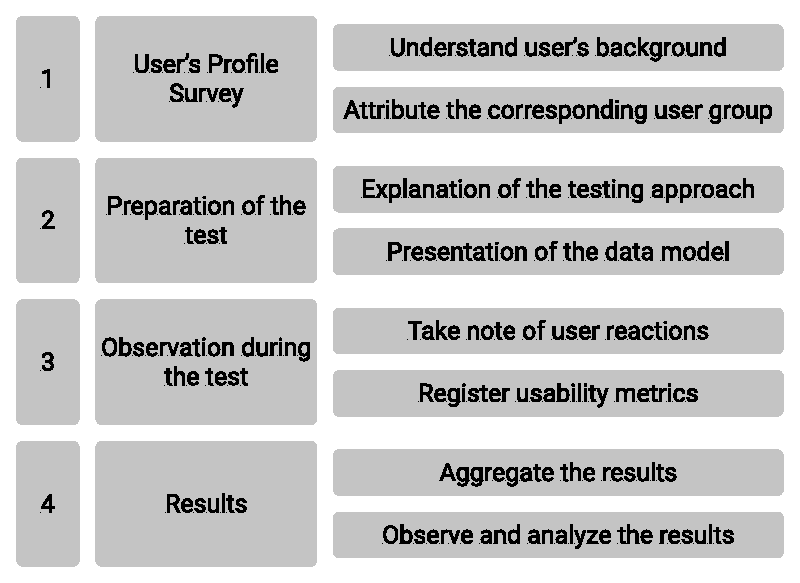
\includegraphics[height=2.4in]{evaluation-method-diagram}
	\caption{Evaluation method overview.}
	\label{fig:evaluationMethodDiagram}
\end{figure}


\medskip
\textbf{Understanding the user's profile:}
\medskip

All users tested, started by filling a survey, which included the questions presented in Table \ref{tab:survey_users_profile}, in order to perceive what is their background regarding software development, relational databases, and data management and visualization tools.

% Please add the following required packages to your document preamble:
% \usepackage{booktabs}
\begin{table}[tb]
    \caption{Survey to undertand users' profile}
    \label{tab:survey_users_profile}
    \begin{tabular}{@{}lm{4cm}C{1.3cm}C{1.3cm}C{2cm}C{1.3cm}C{1.4cm}@{}}
    \toprule
    ID & Question                                                        & \multicolumn{5}{l}{Possible answers}                                                                        \\ \midrule
    1  & What is your professional occupation?                           & \multicolumn{5}{l}{Open question}                                                                           \\
    2  & Have you a degree in Computer Science or similar?               & Yes           & No                    & \multicolumn{3}{l}{}                                                \\
    3  & Do you have other academic backgrounds?                         & \multicolumn{5}{l}{Open question}                                                                           \\
    4  & Have you already used OutSystems?                               & Never use     & Almost never          & Occasionally / Sometimes & Almost every time & Frequently use       \\
    5  & How long do you use the platform?                               & No experience & \textless{}= 6 months & \textless{}= 1 year      & 1-3 years         & \textgreater 4 years \\
    6  & Have you used a query language (SQL or other)?                  & Never use     & Almost never          & Occasionally / Sometimes & Almost every time & Frequently use       \\
    7  & When was the last time that you have used SQL to build queries? & Never use     & Some weeks ago        & Some months ago          & Last year         & Some years ago       \\
    8  & From 1 to 5, how do you define your SQL expertise level?        & 1             & 2                     & 3                        & 4                 & 5                    \\
    9  & Have you already used relational databases?                     & Never use     & Almost never          & Occasionally / Sometimes & Almost every time & Frequently use       \\
    10 & Are you familiar with relational operators (joins)?             & Yes           & No                    & \multicolumn{3}{l}{}                                                \\
    11 & How often do you use spreadsheet applications?                  & Never use     & Almost never          & Occasionally / Sometimes & Almost every time & Frequently use       \\
    12 & How often do you use business intelligence software?            & Never use     & Almost never          & Occasionally / Sometimes & Almost every time & Frequently use      
    \end{tabular}
    \end{table}

The answers to these questions were used to identify the profile of each user according to the three user groups defined:

\begin{itemize}
    \item \textbf{Citizen Developer: } users who do not have extensive software development background neither using traditional programming languages nor with low-code platforms;
    \item \textbf{Software Developer: } users experienced using traditional programming languages but not accustomed to use low-code development solutions;
    \item \textbf{OutSystems Developer: } users who have experience developing software with OutSystems, independently of their background.
\end{itemize}

More details regarding the user groups definition will be further provided in section \ref{subsec:user_groups}.

\medskip
\textbf{Preparation of the test:}
\medskip

After perceiving the user's profile, the data model was presented, focusing on the most relevant aspects of the tests. In that way, it was explained how the entities of the model were related with each other and the most used attributes in the scenarios were highlighted. 

Users observed the database diagram illustrated in Figure \ref{fig:dataModel} and a presentation of each entity was provided through a dialogue where the focus was the explanation of the entities included in the data model and how they are related (i.e., explaining which foreign keys were used to link the entities presented). The language used was adapted according to the users' background regarding relational databases. For users who have previous knowledge regarding join operations, it was reinforced the foreign keys used in each join. On the other hand, the explanation to users who did not have previous knowledge in this subject was simplified, explaining for other words what meant the links between entities, providing whenever necessary examples to ensure users understood the data model adopted for tests. As soon as users confirmed that they understood the overview of the existing entities, the testing process started. 

\medskip
\textbf{Observation during the test:}
\medskip

While users were interacting with the system in order to accomplish the proposed scenarios, it was observed the approaches used to solve the problems and the difficulties felt.

However, following users' reasoning and opinions while they interact with the interface was not considered sufficient to collect all necessary results. Therefore, an evaluation methodology was designed to collect the required data using the same approach for all tested interfaces. In that way, Table \ref{tab:scenarios_registered_aspects} enumerates all aspected registered and evaluated in usability tests for each scenario. The aspects listed in this table were registered manually inserted the observation results in a spreadsheet as exemplified in Figure \ref{fig:userEvaluationExample}.

For all scenarios, it was registered the time they needed to perform it as well as if they reached the task goal according to the classification presented in Table \ref{tab:effectiveness_states}. 

In addition, a text highlighting the most relevant usability test topics, including users' opinions, reactions, expectations, and suggestions has been included for each user. It was registered the qualitative result of the usability tests, which are not only important for the design of the next iterations but also to assess users' satisfaction.

%Figure \ref{fig:userEvaluationExample} demonstrates the table used as support to register the duration and success rate of each scenario as well as the general observations summed up at the final of the user test.

%Furthermore, other important details of each scenario were reported. In the comprehension scenarios, it was assessed the correct components of the query identified and the means used to perceive the solution. Regarding the formulation scenarios, the options used to build the query were identified and also the difficulties and the exploration of not supported options.




\begin{figure}[htbp]
	\centering
	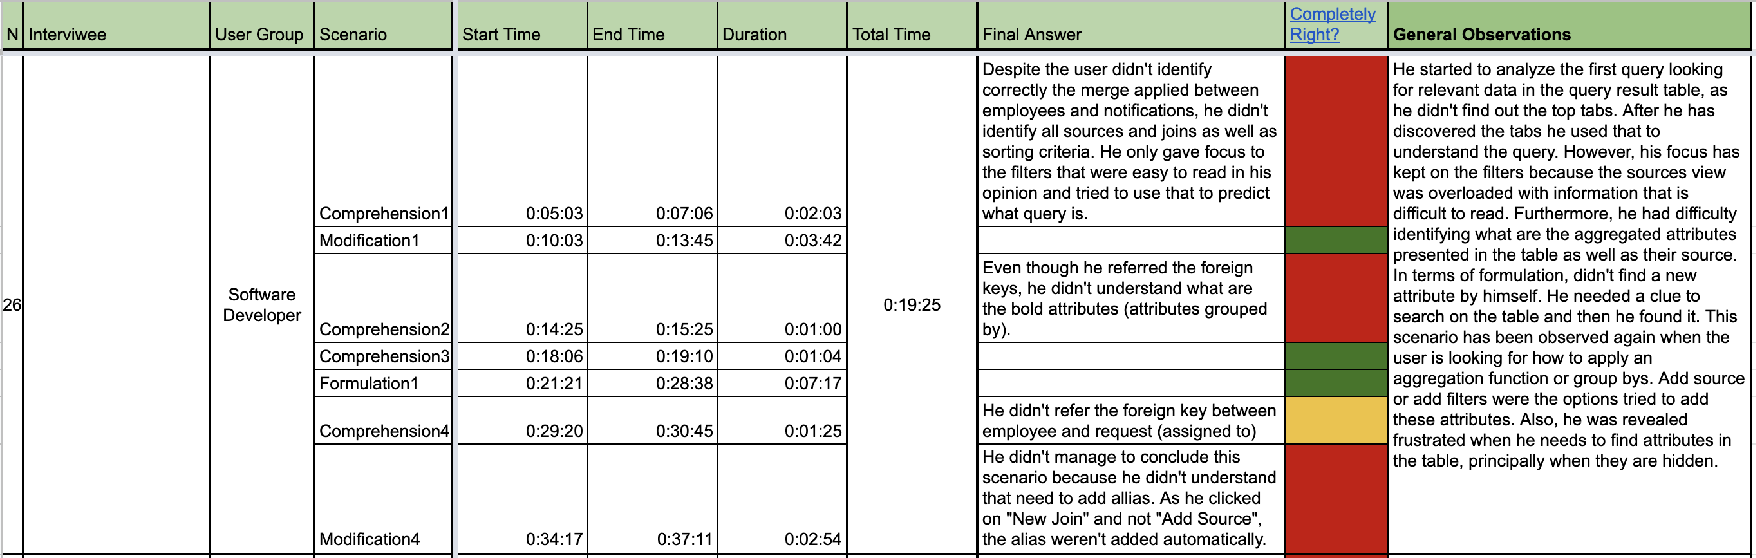
\includegraphics[height=1.9in]{user-evaluation-example}
	\caption{Example of a general annotation registered after a usability test.}
	\label{fig:userEvaluationExample}
\end{figure}


% Please add the following required packages to your document preamble:
% \usepackage{booktabs}
% \usepackage[table,xcdraw]{xcolor}
% If you use beamer only pass "xcolor=table" option, i.e. \documentclass[xcolor=table]{beamer}
% \usepackage{longtable}
% Note: It may be necessary to compile the document several times to get a multi-page table to line up properly
\begin{longtable}{@{}lm{7cm}ccccccc@{}}
    \caption{Evaluation points registered in each scenario.}
    \label{tab:scenarios_registered_aspects}\\
    \toprule
    \rowcolor[HTML]{EFEFEF} 
    \textbf{ID} & \textbf{Scenario}                                                                                                                                       & \multicolumn{1}{l}{\cellcolor[HTML]{EFEFEF}C1} & \multicolumn{1}{l}{\cellcolor[HTML]{EFEFEF}M1} & \multicolumn{1}{l}{\cellcolor[HTML]{EFEFEF}C2} & \multicolumn{1}{l}{\cellcolor[HTML]{EFEFEF}C3} & \multicolumn{1}{l}{\cellcolor[HTML]{EFEFEF}F1} & \multicolumn{1}{l}{\cellcolor[HTML]{EFEFEF}C4} & \multicolumn{1}{l}{\cellcolor[HTML]{EFEFEF}M4} \\* \midrule
    \endfirsthead
    %
    \multicolumn{9}{c}%
    {{\bfseries Table \thetable\ continued from previous page}} \\
    \toprule
    \rowcolor[HTML]{EFEFEF} 
    \textbf{ID} & \textbf{Scenario}                                                                                                                                       & \multicolumn{1}{l}{\cellcolor[HTML]{EFEFEF}C1} & \multicolumn{1}{l}{\cellcolor[HTML]{EFEFEF}M1} & \multicolumn{1}{l}{\cellcolor[HTML]{EFEFEF}C2} & \multicolumn{1}{l}{\cellcolor[HTML]{EFEFEF}C3} & \multicolumn{1}{l}{\cellcolor[HTML]{EFEFEF}F1} & \multicolumn{1}{l}{\cellcolor[HTML]{EFEFEF}C4} & \multicolumn{1}{l}{\cellcolor[HTML]{EFEFEF}M4} \\* \midrule
    \endhead
    %
    \bottomrule
    \endfoot
    %
    \endlastfoot
    %
                & \textbf{General observation aspects}                                                                                                                    &                                                &                                                &                                                &                                                &                                                &                                                &                                                \\* \midrule
    S1          & Task completion                                                                                                                                         & X                                              & X                                              & X                                              & X                                              & X                                              & X                                              & X                                              \\
    S2          & Time used to perform the scenario                                                                                                                       & X                                              & X                                              & X                                              & X                                              & X                                              & X                                              & X                                              \\
    S3 & Components of the interface explored                                                                                                          & X                                              & X                                              & X                                              & X                                              & X                                              & X                                              & X                                              \\* \midrule
                & \textbf{Regarding comprehension scenarios}                                                                                                              &                                                &                                                &                                                &                                                &                                                &                                                &                                                \\* \midrule
    S4          & First area of the interface used to explore the query                                                                                                   & X                                              &                                                & X                                              & X                                              &                                                & X                                              &                                                \\
    S5          & List of the entities identified                                                                                                                         & X                                              &                                                & X                                              & X                                              &                                                & X                                              &                                                \\
    S6          & List of the joins identified                                                                                                                            & X                                              &                                                & X                                              & X                                              &                                                & X                                              &                                                \\
    S7          & In the cases the join is a left join with a condition where the right entity identifier must be null & X                                               &                                                &                                               &                                                &                                                &                                              &                                                \\
    S8          & In the cases the join between two entities could be made using different foreign keys, identification if user identified correctly the foreign key used &                                                &                                                & X                                              &                                                &                                                & X                                              &                                                \\
    S9          & List of the filters identified                                                                                                                          & X                                              &                                                & X                                              &                                                &                                                & X                                              &                                                \\
    S10          & List of the sorting criteria identified                                                                                                                 & X                                              &                                                & X                                              & X                                              &                                                & X                                              &                                                \\* \midrule
                & \textbf{Regarding modification scenarios}                                                                                                               &                                                &                                                &                                                &                                                &                                                &                                                &                                                \\* \midrule
    S11         & Task completion of the required modification of the existing filters                                                                                    &                                                & X                                              &                                                &                                                &                                                &                                                &                                                \\
    S12         & Time needed to perform the required modification of the existing filters                                                                                &                                                & X                                              &                                                &                                                &                                                &                                                &                                                \\
    S13         & Registered if users made mistaked when they were changing the required filters                                                                          &                                                & X                                              &                                                &                                                &                                                &                                                &                                                \\
    S14         & Task completion of the insertion of the required calculated attribute                                                                                   &                                                & X                                              &                                                &                                                &                                                &                                                &                                                \\
    S15         & Time spent to add the required calculated attribute                                                                                                     &                                                & X                                              &                                                &                                                &                                                &                                                &                                                \\
    S16         & Option used to add the required calculated attribute                                                                                                    &                                                & X                                              &                                                &                                                &                                                &                                                &                                                \\
    S17         & Alternative options tried in order to find how to add the required calculated attribute                                                                 &                                                & X                                              &                                                &                                                &                                                &                                                &                                                \\
    S18         & Registered if users had difficulties to find how to add the required calculated attribute                                                               &                                                & X                                              &                                                &                                                &                                                &                                                &                                                \\
    S19         & Registered if users needed a clue in order to find how to add the required calculated attribute                                                         &                                                & X                                              &                                                &                                                &                                                &                                                &                                                \\* \midrule
                & \textbf{Regarding formulation scenario}                                                                                                                 &                                                &                                                &                                                &                                                &                                                &                                                &                                                \\* \midrule
    S20         & List of entities inserted                                                                                                                               &                                                &                                                &                                                &                                                & X                                              &                                                &                                                \\
    S21         & List of joins inserted                                                                                                                                  &                                                &                                                &                                                &                                                & X                                              &                                                &                                                \\
    S22         & Selection of the required foreign key in the cases where the join between two entities could be made using different foreign keys                       &                                                &                                                &                                                &                                                & X                                              &                                                &                                                \\
    S23         & Registered if users managed to add the required group filter                                                                                            &                                                &                                                &                                                &                                                & X                                              &                                                &                                                \\
    S24         & Task completion of the addition of the required aggregated attributes                                                                                                   &                                                &                                                &                                                &                                                & X                                              &                                                &                                                \\
    S25         & Time needed to add the required aggregated attributes                                                                                                   &                                                &                                                &                                                &                                                & X                                              &                                                &                                                \\
    S26         & Option used to add the required aggregated attributes                                                                                                   &                                                &                                                &                                                &                                                & X                                              &                                                &                                                \\
    S27         & Alternative options tried in order to find how to add the required aggregated attributes                                                                &                                                &                                                &                                                &                                                & X                                              &                                                &                                                \\
    S28         & Registered if users had difficulties to find how to add the required aggregated attributes                                                              &                                                &                                                &                                                &                                                & X                                              &                                                &                                                \\
    S29         & Registered if users needed a clue in order to find how to add the required aggregated attributes                                                        &                                                &                                                &                                                &                                                & X                                              &                                                &                                                \\* \bottomrule
    \end{longtable}



\begin{table}[tb]
        \caption{Description of the effectiveness states considered.}
        \label{tab:effectiveness_states}
        \begin{tabular}{|l|l|l|l|}
            \hline
            \rowcolor[HTML]{C0C0C0} 
            \textbf{Legend}                                                                                                 & \textbf{Comprehension}                                                                                                                                                                                                                                                                                                             & \textbf{Modification}                                                  & \textbf{Formulation}                                                                   \\ \hline
            \cellcolor[HTML]{38761D}{\color[HTML]{FFFFFF} \textbf{Achieved}}                                                & \begin{tabular}[c]{@{}l@{}}When the user mentioned \\ all components of the queries \\ (sources, joins with foreign \\ keys, filters, sorting, aggregation \\ functions). The only thing that \\ would not be considered is if \\ the user didn't refer with or \\ without joins when they were \\ put automatically.\end{tabular} & All modifications                                                      & \begin{tabular}[c]{@{}l@{}}Completely \\ Right\end{tabular}                            \\ \hline
            \cellcolor[HTML]{F1C232}\textbf{\begin{tabular}[c]{@{}l@{}}Partially \\ Achieved\end{tabular}}                  & \begin{tabular}[c]{@{}l@{}}If the user didn't refer to the \\ foreign key between two tables \\ where there is more than one \\ foreign key between two tables. \\ The another possibility is if the \\ user did not specify only the \\ sorting criteria.\end{tabular}                                                            & \begin{tabular}[c]{@{}l@{}}Forgot to remove\\ some filter\end{tabular} & \begin{tabular}[c]{@{}l@{}}Group data \\ using the \\ wrong \\ identifier\end{tabular} \\ \hline
            \cellcolor[HTML]{CC0000}{\color[HTML]{FFFFFF} \textbf{\begin{tabular}[c]{@{}l@{}}Not \\ Achieved\end{tabular}}} & Anything else                                                                                                                                                                                                                                                                                                                      & Anything else                                                          & Anything else                                                                          \\ \hline
            \end{tabular}
        \end{table}


\medskip
\textbf{Evaluation of the users' satisfaction after using the interface:}
\medskip

Finally, to gain a more extensive notion and some quantitative metrics about the interaction with the interfaces, the users were asked to fill in a System Usability Scale (SUS) \cite{system_usability_scale} as their final task in the usability test, where users needed to classify the questions bellow with a number from 1 (strongly disagree) to 5 (strongly agree):

\begin{enumerate}
    \item I think that I would like to use this system frequently;
    \item I found the system unnecessarily complex;
    \item I thought the system was easy to use;
    \item I think that I would need the support of a technical person to be able to use this system;
    \item I found the various functions in this system were well integrated;
    \item I thought there was too much inconsistency in this system;
    \item I would imagine that most people would learn to use this system very quickly;
    \item I found the system very cumbersome to use;
    \item I felt very confident using the system;
    \item I needed to learn a lot of things before I could get going with this system.
\end{enumerate}

The process detailed in this chapter was used in all interfaces tested and addressed in this dissertation: the existing interface of Aggregates, the paper prototype, and the final prototype which was integrated into Service Studio (the Visual \gls{IDE} of the OutSystems Platform). 

\section{Summary}
\label{sec:summary}
Figure \ref{fig:methodologyOverview} summarizes the methodology described in this chapter, from the problem definition to the final prototype implemented. As can be observed, there were two major phases throughout this dissertation:

\begin{itemize}
    \item \textbf{Requirements and Analysis: } The stage where the problem was defined as well as the target users of the system were identified and classified into different groups according to their requirements and expectations. The output of these two analyses was taken into account to prepare the user testing environment so that the scenarios and the evaluation method were defined;
    \item \textbf{Design and Implementation: } The process to reach the redesigned interface, from the first sketchings to the final prototype integrated into the Service Studio code. The results of each phase were taken into account in the following phase, in order to evaluate the design choices made gradually.
\end{itemize}

Finally, the results of the user testing of the final prototype were compared against the results obtained when users tested the existing interface in order to measure the success of the prototype built.

\begin{figure}[htbp]
	\centering
	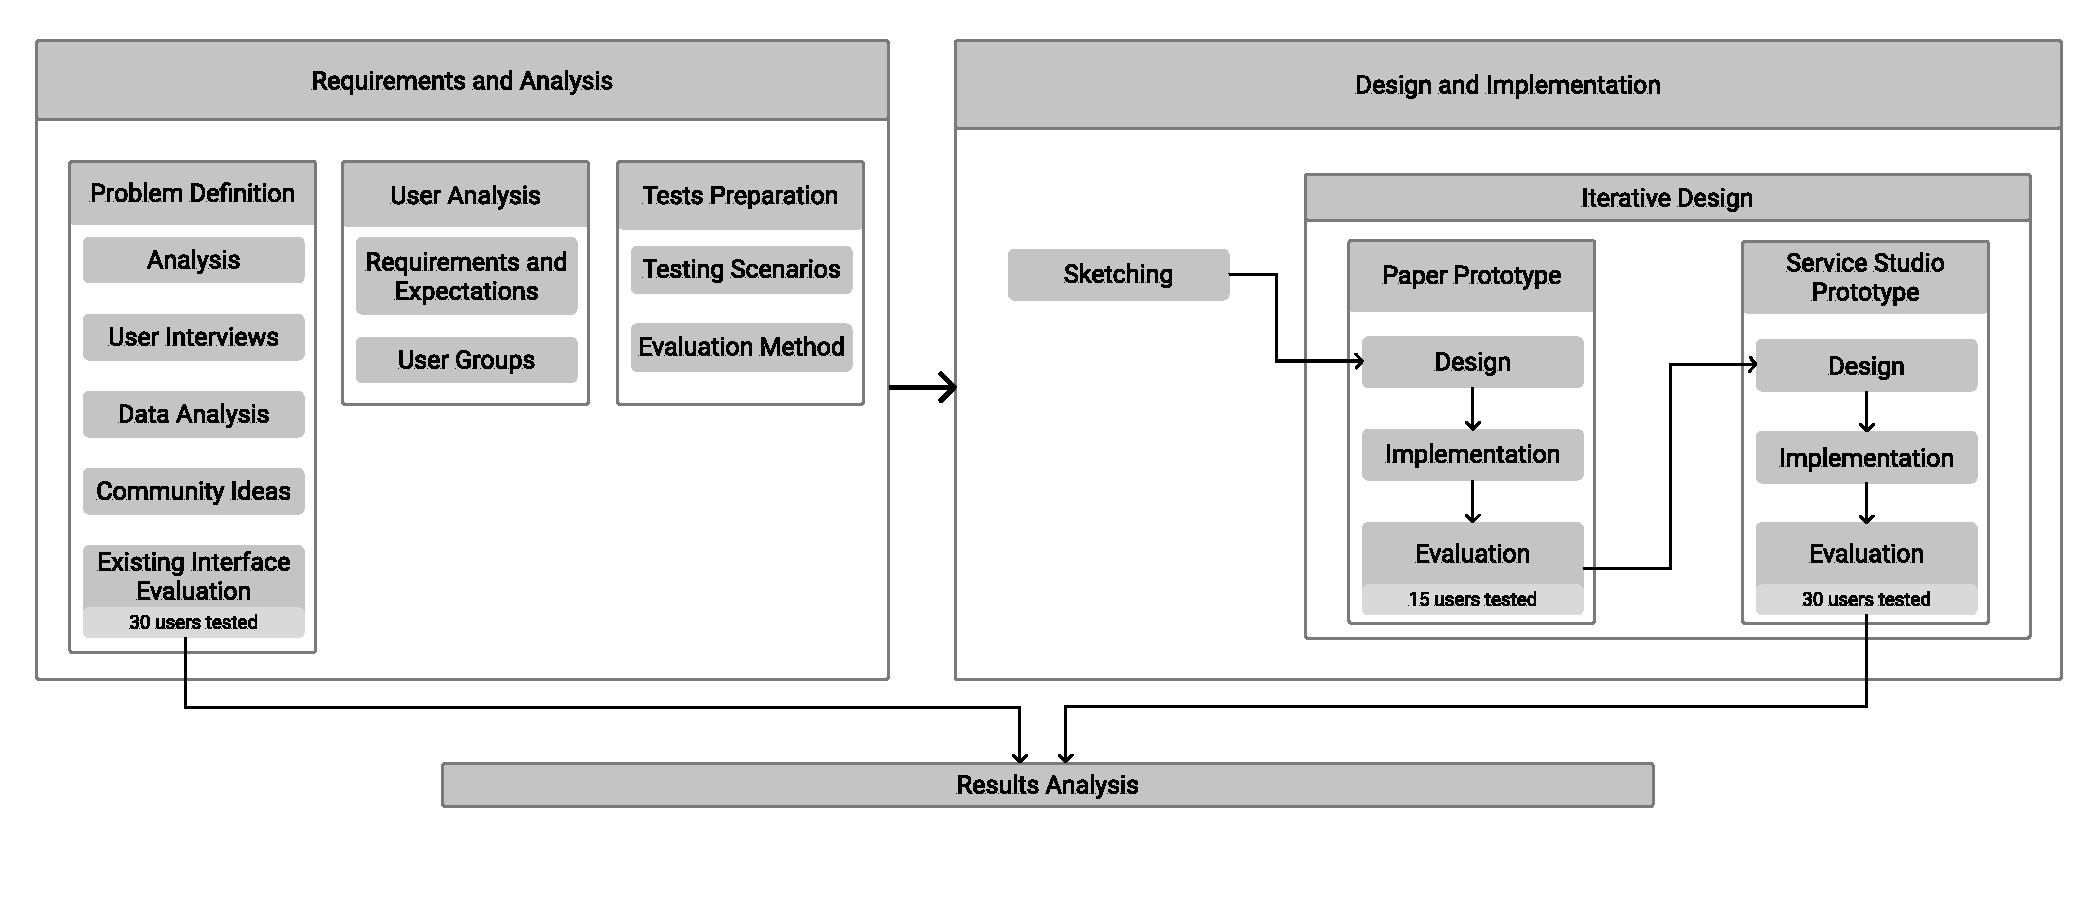
\includegraphics[height=2.6in]{methodology-overview}
	\caption{Methodology Overview}
	\label{fig:methodologyOverview}
\end{figure}